\documentclass[aspectratio=169,11pt]{beamer}
\usetheme[progressbar=frametitle,numbering=fraction]{metropolis}
\usepackage{booktabs}
\usepackage{tikz}
\usetikzlibrary{positioning,arrows.meta,calc}
\graphicspath{{../report/figures/}}

\definecolor{accent}{HTML}{2A78D6}
\definecolor{warm}{HTML}{EB6834}
\definecolor{good}{HTML}{0CA30C}
\setbeamercolor{alerted text}{fg=warm}
\setbeamercolor{frametitle}{bg=black!80}

\tikzset{
  box/.style={draw=black!40, rounded corners=2pt, fill=accent!8, align=center, font=\small, minimum height=9mm, text width=24mm},
  hot/.style={box, fill=warm!12},
  arr/.style={-{Stealth[length=2mm]}, thick, black!60}}

\newcommand{\bignum}[1]{{\Large\bfseries #1}}

\title{How Much of the Reported Performance Survives?}
\subtitle{Reproducing and extending a hybrid ensemble model for APT attack detection}
\author{Achyutananda Sahoo, [team member], [team member]}
\institute{Research in Information Security \quad$\cdot$\quad IIIT Hyderabad}
\date{Monsoon 2026}

\begin{document}

\maketitle

% ------------------------------------------------------------------
\begin{frame}{Why APTs are hard to catch}
\begin{columns}[T]
\column{0.55\textwidth}
\begin{itemize}
  \item \textbf{Advanced Persistent Threats} are slow, targeted intrusions that can stay hidden for months
  \item They blend into normal traffic, so \alert{signature-based} defences (antivirus, firewalls, rule IDSs) miss them
  \item \textbf{Network behaviour anomaly detection}: learn what normal flows look like and flag deviations
  \item Machine learning on labelled flow records is the standard way to learn that boundary
\end{itemize}
\column{0.4\textwidth}
\vspace{6mm}
\begin{center}
\bignum{Years}\\[2pt]
{\small how long the spyware in the paper's example (linked to APT27 and APT41) went unnoticed}\\[14pt]
\bignum{0.1\% $\times$ 1M}\\[2pt]
{\small a 0.1\% false-alarm rate on a million flows a day means 1{,}000 alerts a day}
\end{center}
\end{columns}
\end{frame}

% ------------------------------------------------------------------
\begin{frame}{The paper in one slide}
\begin{columns}[c]
\column{0.52\textwidth}
\begin{center}
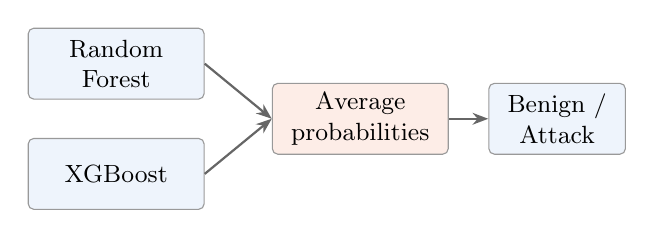
\begin{tikzpicture}
\node[box, text width=20mm] (rf) at (0, 0.7) {Random Forest};
\node[box, text width=20mm] (xgb) at (0, -0.7) {XGBoost};
\node[hot, text width=20mm] (avg) at (3.1, 0) {Average\\probabilities};
\node[box, text width=15mm] (out) at (5.6, 0) {Benign /\\Attack};
\draw[arr] (rf.east) -- (avg.west); \draw[arr] (xgb.east) -- (avg.west); \draw[arr] (avg) -- (out);
\end{tikzpicture}
\end{center}
\begin{itemize}\small
  \item All attacks merged into one ``anomaly'' class
  \item SMOTE-Tomek, Pearson + mutual-information feature selection, SHAP
\end{itemize}
\column{0.45\textwidth}
\centering\textbf{Reported accuracy of the hybrid}\\[4pt]
\begin{tabular}{lr}
\toprule
CSE-CIC-IDS2018 & 98.92\% \\
CIC-IDS2017     & 99.91\% \\
NSL-KDD         & 99.24\% \\
UNSW-NB15       & 97.11\% \\
\bottomrule
\end{tabular}\\[6pt]
{\small Best of 13 models on every dataset}
\end{columns}
\vspace{4mm}
{\footnotesize Saini, Bhat Kasaragod, Prakasha \& Das (2023), \emph{Concurrency and Computation: Practice and Experience}}
\end{frame}

% ------------------------------------------------------------------
\begin{frame}{What we set out to do}
\begin{columns}[T]
\column{0.32\textwidth}
\textcolor{accent}{\textbf{1. Reproduce}}\\[4pt]
\small Rebuild the full pipeline on all four datasets and compare every number with the paper
\column{0.32\textwidth}
\textcolor{accent}{\textbf{2. Extend}}\\[4pt]
\small Test what the paper names as future work: a \emph{trained} combiner with a deep model, plus a modern tabular transformer
\column{0.32\textwidth}
\textcolor{accent}{\textbf{3. Scrutinise}}\\[4pt]
\small Ask whether the 97--99.9\% holds up, and why it might not
\end{columns}
\vspace{10mm}
\begin{center}
\small Everything runs from one configurable codebase on Kaggle (T4 GPU):\\
\texttt{github.com/Sahoo-Achyutananda/RIS-M26}
\end{center}
\end{frame}

% ------------------------------------------------------------------
\section{Data and pipeline}

\begin{frame}{Four datasets, very different shapes}
\centering
\begin{tabular}{lrrrl}
\toprule
Dataset & Raw rows & Attack share & Rows used & Sampling \\
\midrule
NSL-KDD          & 148{,}517      & 48\% & 147{,}888 & none \\
UNSW-NB15        & 257{,}673      & 64\% & 154{,}098 & none \\
CIC-IDS2017      & $\approx$2.83M & 20\% & 49{,}235  & 2\% per file \\
CSE-CIC-IDS2018  & 16.2M          & 17\% & 30{,}838  & 0.2\% per file \\
\bottomrule
\end{tabular}
\vspace{6mm}
\begin{itemize}\small
  \item \textbf{We explored the raw files first}, before writing any cleaning code
  \item What we found: header rows repeated inside the data, the literal text \texttt{Infinity}, 40\% duplicate rows in
        UNSW-NB15, a label column hiding among the features, and a 3.9\,GB file with extra columns
\end{itemize}
\end{frame}

\begin{frame}{What the raw data looked like: CSE-CIC-IDS2018}
\centering
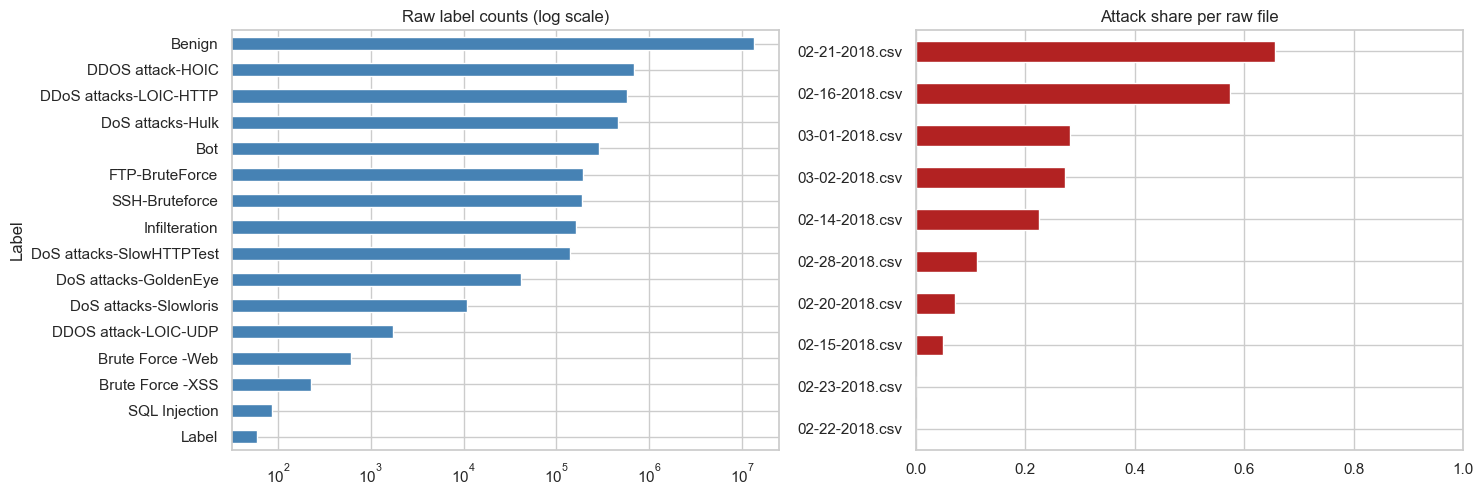
\includegraphics[width=0.95\textwidth]{eda_cse_cic_ids2018_classes.png}\\[2pt]
\small Left: 16.2M flows, 14 attack types, plus a ``Label'' class (the header repeated 59 times).
Right: the attack share swings from 0\% to 66\% between daily files.
\end{frame}

\begin{frame}{Our pipeline}
\centering
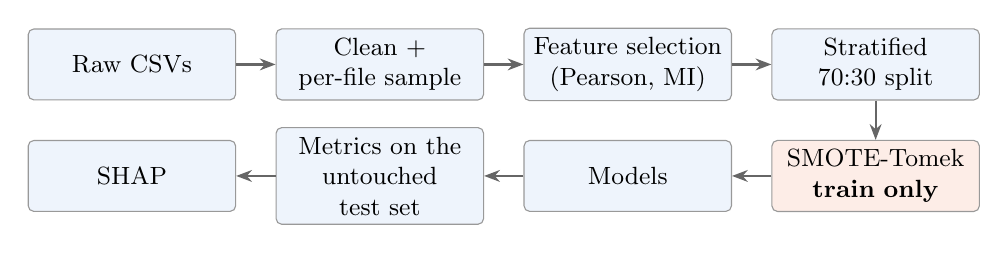
\begin{tikzpicture}[node distance=5mm and 5mm]
\node[box] (raw) {Raw CSVs};
\node[box, right=of raw] (clean) {Clean +\\per-file sample};
\node[box, right=of clean] (fs) {Feature selection\\(Pearson, MI)};
\node[box, right=of fs] (split) {Stratified\\70:30 split};
\node[hot, below=of split] (bal) {SMOTE-Tomek\\\textbf{train only}};
\node[box, left=of bal] (models) {Models};
\node[box, left=of models] (eval) {Metrics on the\\untouched test set};
\node[box, left=of eval] (shap) {SHAP};
\draw[arr] (raw) -- (clean); \draw[arr] (clean) -- (fs); \draw[arr] (fs) -- (split);
\draw[arr] (split) -- (bal); \draw[arr] (bal) -- (models); \draw[arr] (models) -- (eval); \draw[arr] (eval) -- (shap);
\end{tikzpicture}
\vspace{6mm}
\begin{itemize}\small
  \item \textbf{Models:} Decision Tree, Logistic Regression, MLP, Random Forest, XGBoost, and the paper's averaging hybrid
  \item \textbf{One deliberate difference:} the paper balances \emph{before} splitting, so synthetic samples built from
        test rows leak into training. We balance the training split only
\end{itemize}
\end{frame}

\begin{frame}{Detective work: an undocumented step}
\begin{columns}[c]
\column{0.5\textwidth}
\begin{itemize}\small
  \item The paper describes sampling only for CSE-CIC-IDS2018
  \item Yet its CIC-IDS2017 table has $\approx$56.6k rows, from a dataset of 2.83M
  \item Dividing its class counts by the raw counts:
\end{itemize}
\vspace{2mm}
\centering\bignum{Exactly 2\%} \\ {\small for every attack class}
\column{0.46\textwidth}
\centering
\begin{tabular}{lrrr}
\toprule
Class & Raw & Paper & Ratio \\
\midrule
PortScan    & 158{,}930 & 3{,}179 & 2.00\% \\
DDoS        & 128{,}027 & 2{,}561 & 2.00\% \\
FTP-Patator & 7{,}938   & 159     & 2.00\% \\
SSH-Patator & 5{,}897   & 118     & 2.00\% \\
Bot         & 1{,}966   & 39      & 1.98\% \\
\bottomrule
\end{tabular}\\[6pt]
{\small The same check showed we were missing the Wednesday (DoS) file}
\end{columns}
\end{frame}

% ------------------------------------------------------------------
\section{Results}

\begin{frame}{Reproduction: the paper's hybrid, reported vs.\ ours}
\centering
\begin{tabular}{lcccc}
\toprule
& \multicolumn{2}{c}{Accuracy} & \multicolumn{2}{c}{False-positive rate} \\
\cmidrule(lr){2-3}\cmidrule(lr){4-5}
Dataset & Paper & Ours & Paper & Ours \\
\midrule
NSL-KDD         & 99.24 & 99.60 & 0.62 & \textcolor{good}{0.33} \\
CSE-CIC-IDS2018 & 98.92 & 98.59 & 0.52 & \textcolor{good}{0.38} \\
CIC-IDS2017     & 99.91 & 99.86 & 0.12 & \textcolor{good}{0.10} \\
UNSW-NB15       & 97.11 & \alert{91.33} & 5.29 & \alert{8.94} \\
\bottomrule
\end{tabular}
\vspace{6mm}
\begin{itemize}\small
  \item \textbf{3 of 4 datasets reproduce} within 0.36 points, with a lower false-positive rate on all three
  \item The paper's model ranking holds: tree ensembles on top, the hybrid best or within 0.01 points of the best
\end{itemize}
\end{frame}

\begin{frame}{The one big gap: UNSW-NB15}
\begin{columns}[c]
\column{0.5\textwidth}
\centering
\begin{tabular}{lc}
\toprule
Setting & Accuracy \\
\midrule
Duplicates removed (ours) & 91.33 \\
Duplicates kept           & 94.05 \\
Paper                     & 97.11 \\
\bottomrule
\end{tabular}
\column{0.46\textwidth}
\begin{itemize}\small
  \item 40\% of UNSW-NB15 rows are exact duplicates
  \item Kept duplicates can sit in both train and test, so the model is partly tested on data it memorised
  \item Keeping them recovers \textbf{2.7 of the 5.8 points}
  \item The rest: balancing before the split, and an undescribed subset (the paper uses $\approx$81k of 257k rows)
\end{itemize}
\end{columns}
\end{frame}

\begin{frame}{Our extensions}
\begin{columns}[T]
\column{0.5\textwidth}
\textcolor{accent}{\textbf{Stacked hybrid}}\\[4pt]
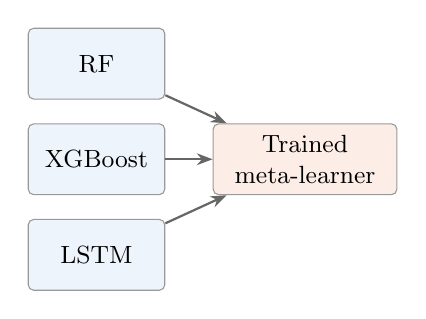
\begin{tikzpicture}[node distance=3mm and 6mm]
\node[box, text width=15mm] (rf) {RF};
\node[box, text width=15mm, below=of rf] (xgb) {XGBoost};
\node[box, text width=15mm, below=of xgb] (lstm) {LSTM};
\node[hot, right=of xgb, text width=21mm] (meta) {Trained\\meta-learner};
\draw[arr] (rf) -- (meta); \draw[arr] (xgb) -- (meta); \draw[arr] (lstm) -- (meta);
\end{tikzpicture}\\[4pt]
\small The paper's future work: combine ML and deep learning, and \emph{learn} the combination instead of a fixed 50/50
average (trained on out-of-fold predictions)
\column{0.5\textwidth}
\textcolor{accent}{\textbf{FT-Transformer}}\\[4pt]
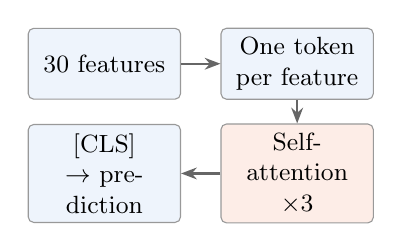
\begin{tikzpicture}[node distance=3mm and 5mm]
\node[box, text width=17mm] (feat) {30 features};
\node[box, text width=17mm, right=of feat] (tok) {One token\\per feature};
\node[hot, text width=17mm, below=of tok] (att) {Self-attention\\$\times 3$};
\node[box, text width=17mm, left=of att] (cls) {[CLS]\\$\rightarrow$ prediction};
\draw[arr] (feat) -- (tok); \draw[arr] (tok) -- (att); \draw[arr] (att) -- (cls);
\end{tikzpicture}\\[4pt]
\small A modern deep model built for tabular data (Gorishniy et al., 2021); unlike an LSTM, it does not pretend the
features have an order
\end{columns}
\end{frame}

\begin{frame}{Extension results \hfill {\normalsize\normalfont same train/test split for every model}}
\centering
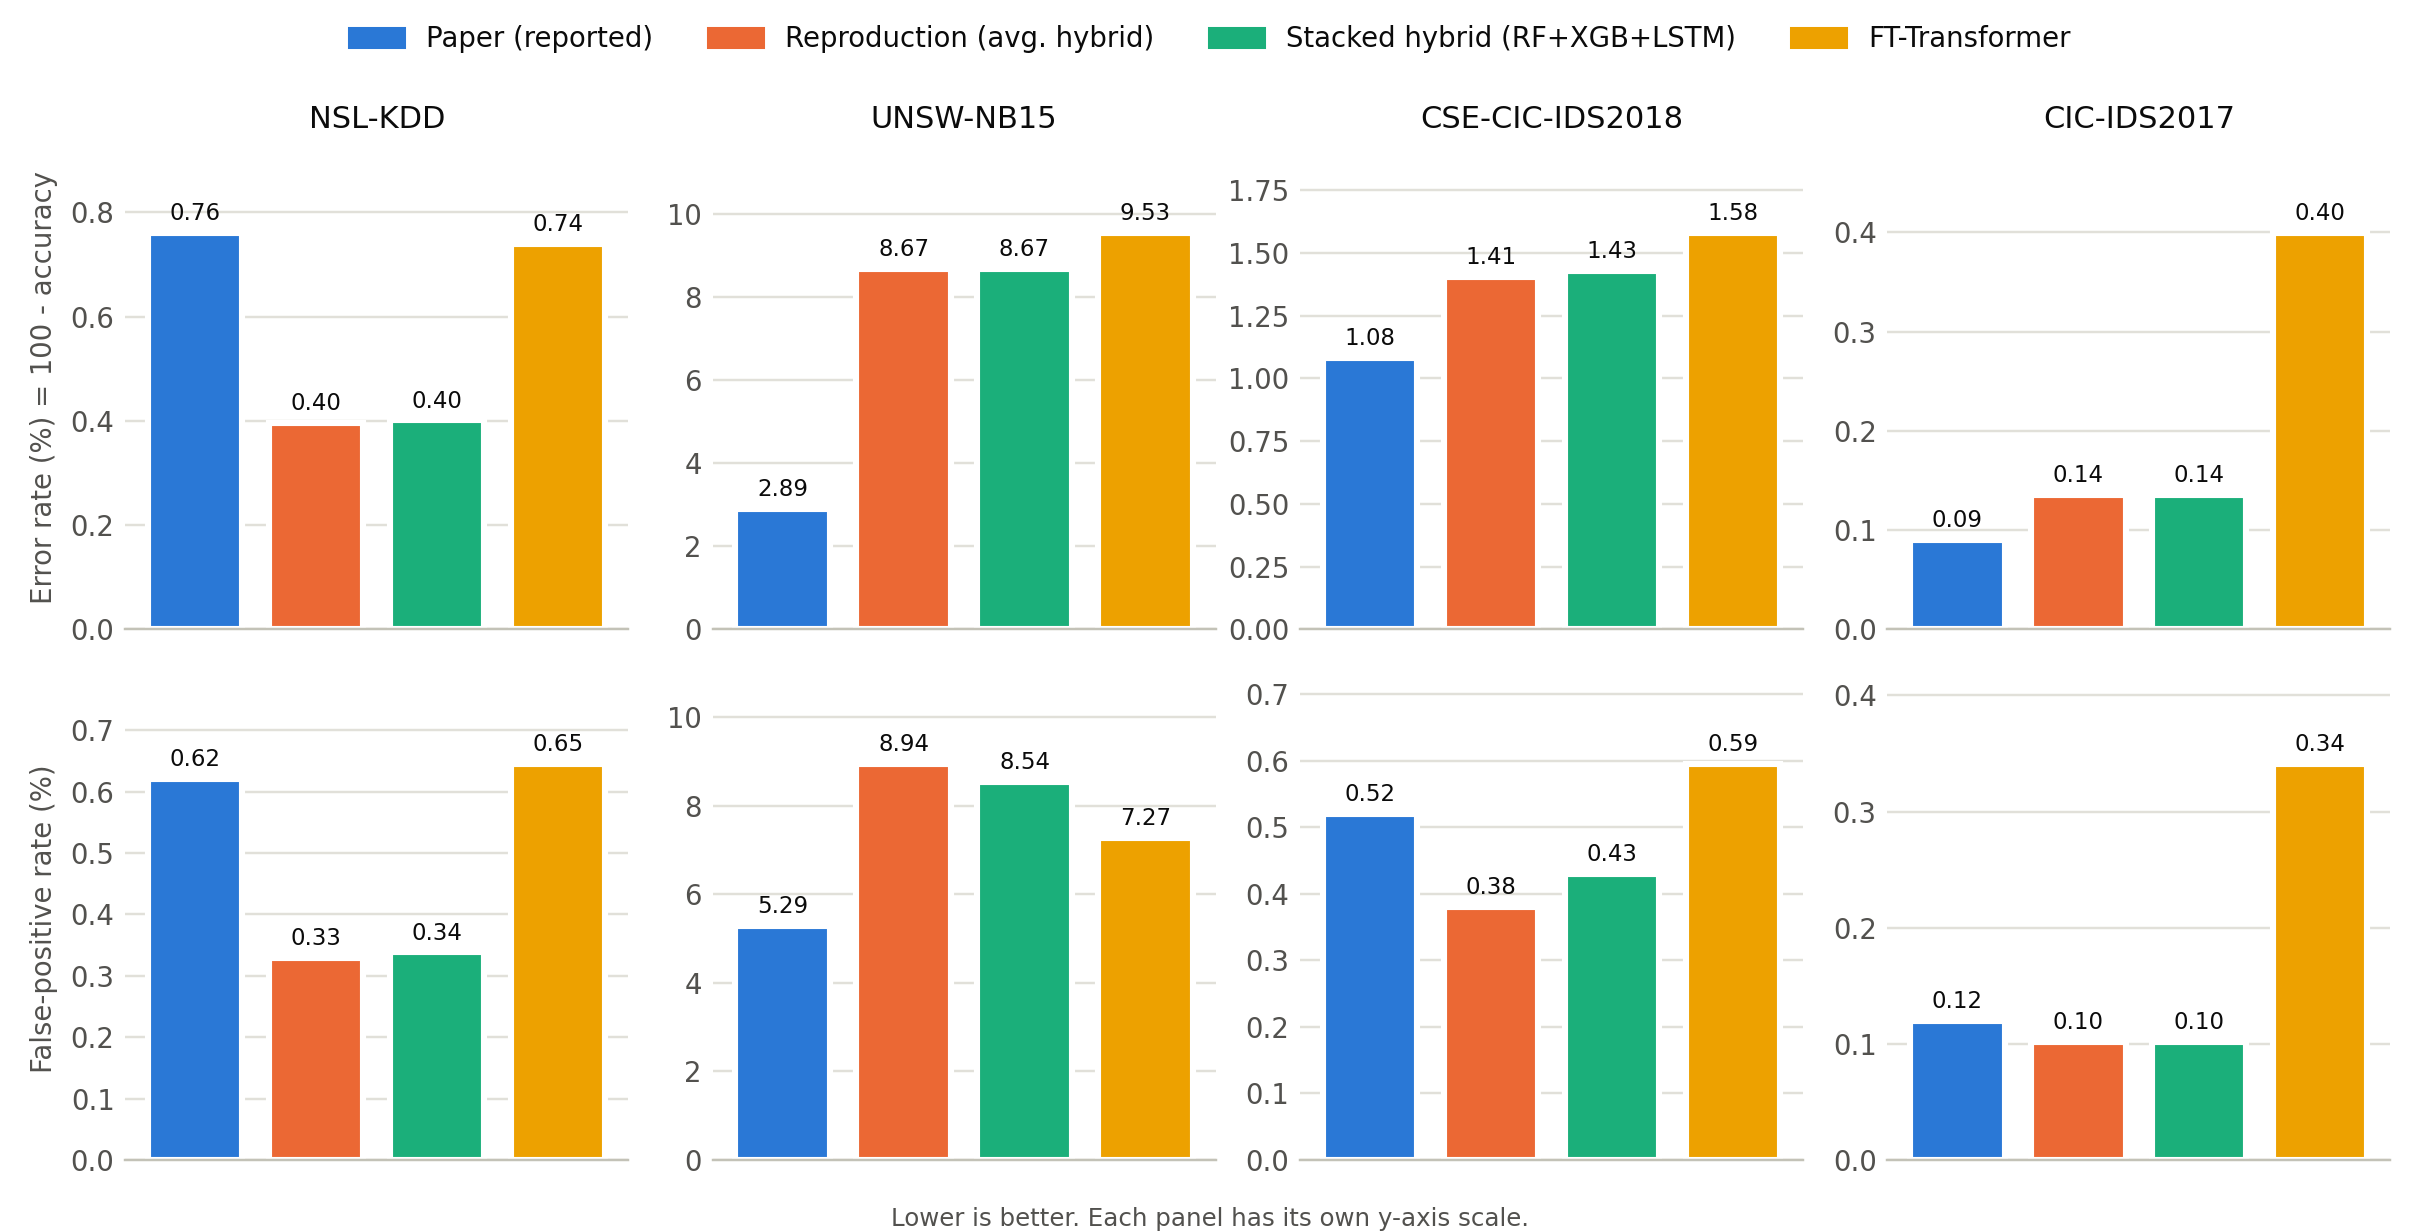
\includegraphics[width=0.93\textwidth]{results_error_fpr.png}
\end{frame}

% ------------------------------------------------------------------
\section{What we learned}

\begin{frame}{Three findings}
\begin{enumerate}
  \item \textbf{The hybrid's advantage is negligible.}\\
        \small On CIC-IDS2017 it beats XGBoost alone by \alert{one flow out of 14{,}771}. On NSL-KDD, XGBoost alone is
        slightly ahead.
        \vspace{3mm}
  \item \textbf{Stacking collapses to averaging.}\\
        \small On CIC-IDS2017 the stacked model makes \alert{exactly the same predictions} as the paper's average.
        The learned combination behaves like plain RF + XGBoost averaging: the LSTM is too weak to matter, and RF and XGBoost
        make the same mistakes.
        \vspace{3mm}
  \item \textbf{Trees still beat the transformer.}\\
        \small The FT-Transformer is 0.2--0.9 points behind on accuracy, but has the \alert{lowest false-positive rate}
        on UNSW-NB15. It makes different errors, so it is the better partner for stacking.
\end{enumerate}
\end{frame}

\begin{frame}{Issues we found in the paper \hfill {\normalsize\normalfont each checkable in the paper itself}}
\begin{itemize}\small
  \item \textbf{Balancing before splitting} (p.~10): synthetic samples from test rows enter training
  \item \textbf{Undocumented 2\% sampling} of CIC-IDS2017
  \item \textbf{Split ratio}: the text says 70:30; the pseudocode says 80:20
  \item \textbf{Identical deep-learning rows}: CNN, ANN and MLP results match to two decimals on NSL-KDD and
        UNSW-NB15, two completely different datasets
  \item \textbf{An impossible F1}: precision 93.84 and recall 99.66 imply F1 $\approx$ 96.66, not the reported 99.66
  \item \textbf{ROC curves made of two straight segments}, the shape of curves drawn from hard 0/1 predictions
  \item \textbf{No variance}: no cross-validation, seeds or significance tests, yet many gains are $<$0.3 points
\end{itemize}
\end{frame}

\begin{frame}{Limitations and next steps}
\begin{columns}[T]
\column{0.47\textwidth}
\textcolor{warm}{\textbf{Our own limitations}}
\begin{itemize}\small
  \item Feature selection also sees the whole dataset
  \item NSL-KDD: random split, not the harder official test set
  \item Single seed, no confidence intervals
  \item No dataset contains real multi-stage APT campaigns
\end{itemize}
\column{0.5\textwidth}
\textcolor{accent}{\textbf{Next phase}}
\begin{itemize}\small
  \item \textbf{Leakage-free protocol}: balancing and feature selection inside each training fold; official NSL-KDD
        test sets
  \item \textbf{Rigour}: multiple seeds, cross-validation, McNemar tests
  \item \textbf{Generalisation}: train on 2017, test on 2018; hold out an attack type as a ``zero-day''
  \item \textbf{Shortcut check}: remove \texttt{Dst Port} and \texttt{Init Fwd Win Byts}
\end{itemize}
\end{columns}
\end{frame}

\begin{frame}[standout]
The paper's numbers largely reproduce,\\
but its hybrid adds almost nothing.\\[10pt]
{\normalsize Next: how much survives a leakage-free evaluation?}\\[16pt]
Thank you. Questions?
\end{frame}

\end{document}
